\section{Import/Export From Other Formats}
\label{sec:pgfplots:importexport}
This section contains information of how to single pictures into separate \pdf\ graphics files (or \eps\ graphics files). Furthermore, it explains a matlab (tm) script which allows to convert from matlab to \PGFPlots.

\subsection[Export to pdf/eps]{Export to {\normalfont\pdf/\eps}}
\label{sec:pgfplots:export}
It is possible to export images to single \pdf-documents using routines of \pgfname\ and/or \Tikz.

\subsubsection[Using the Externalization Framework of PGF By Hand]{Using the Externalization Framework of {\normalfont\pgfname} ``By Hand''}
The first way to export \TeX-pictures to single graphics files is to use the externalization framework of \pgfname.
The basic idea is to encapsulate the desired parts with

\declareandlabel{\beginpgfgraphicnamed}\marg{output file name}

\meta{picture contents}

\declareandlabel{\endpgfgraphicnamed}. 

\noindent Furthermore, one needs to tell \pgfname\ the name of the main document using

\declareandlabel{\pgfrealjobname}\marg{the real job's name}

\noindent in the preamble. This enables two different modes: 
\begin{enumerate}
	\item The first is the normal typesetting mode. \LaTeX\ checks whether a file named \marg{output file name} with one of the accepted file extensions exists -- if that is the case, the graphics file is included with |\pgfimage| and the \meta{picture contents} is skipped. If no such file exists, the \meta{picture contents} is typeset normally. This mode is applied if |\jobname| equals \marg{the real job's name}.
	\item The second mode applies if |\jobname| equals \marg{output file name}, it initiates the ``conversion mode'' which is used to write the graphics file \marg{output file name}. In this case, \emph{only} \meta{picture contents} is written to |\jobname|, the complete rest of the \LaTeX\ is processed as normal, but it is silently discarded.

	This mode needs to be started manually with |pdflatex --jobname |\meta{output file name} for every externalized graphics file.
\end{enumerate}
A complete example may look as follows.
\begin{codeexample}[code only]
\documentclass{article}

\usepackage{pgfplots}

\pgfrealjobname{test}

\begin{document}
	\begin{figure}
		\beginpgfgraphicnamed{testfigure}
		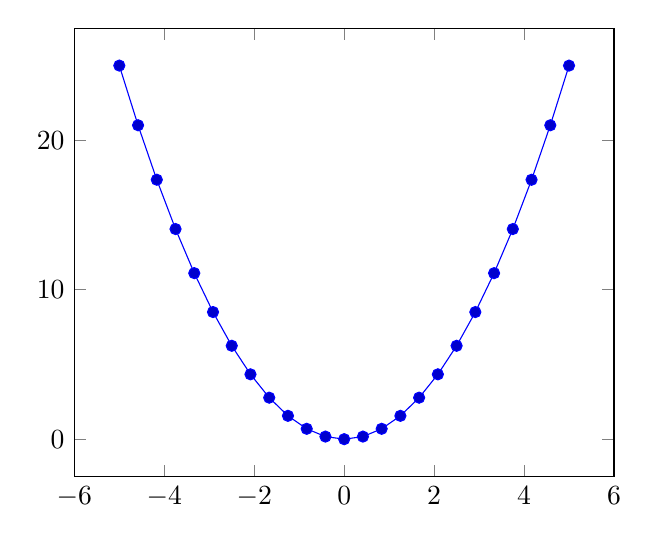
\begin{tikzpicture}
		\begin{axis}
			\addplot {x^2};
		\end{axis}
		\end{tikzpicture}
		\endpgfgraphicnamed
	\caption{Our first external graphics example}
	\end{figure}

	\begin{figure}
		\beginpgfgraphicnamed{testfigure2}
		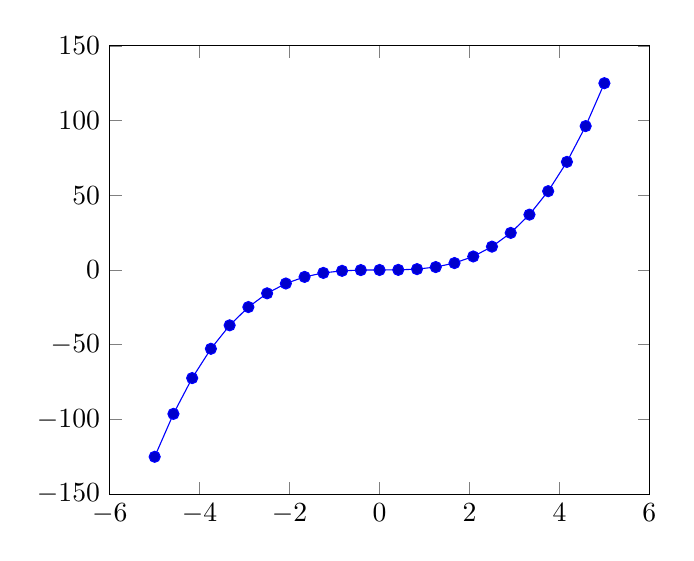
\begin{tikzpicture}
		\begin{axis}
			\addplot {x^3};
		\end{axis}
		\end{tikzpicture}
		\endpgfgraphicnamed
	\caption{A second graphics}
	\end{figure}
\end{document}
\end{codeexample}
\noindent The file is named |test.tex|, and it is processed (for example) with
\begin{codeexample}[code only]
pdflatex test	
\end{codeexample}
\noindent Now, we type
\begin{codeexample}[code only]
pdflatex --jobname testfigure test	
pdflatex --jobname testfigure2 test	
\end{codeexample}
\noindent to enter conversion mode. These last calls will \emph{only} write the contents of our named graphics environments, one for \marg{testfigure} and one for \marg{testfigure2} into the respective output files |testfigure.pdf| and |testfigure2.pdf|.

In summary, one needs |\pgfrealjobname| and calls |pdflatex --jobname |\marg{graphics file} for every externalized graphics environment. Please note that it is absolutely necessary to use the syntax above, \emph{not} |\begin{pgfgraphicnamed}|.

These steps are explained in much more detail in Section``Externalizing Graphics'' of~\cite{tikz}.  This reference also contains information about how to typeset such a document without \pgfname\ installed.

I once attempted to write a unix \texttt{bash}--script |pgf2pdf.sh| which simplifies these steps in case that every externalized graphics environment is placed into a separate file |.pgf|. Interested readers find it in the installation tree.

\paragraph{Attention:} Do not forget a correct |\pgfrealjobname| statement! If it is missing, externalization simply won't work. If it is wrong, any call to \LaTeX\ will produce empty output files.

\subsubsection{Using the Automatic Externalization Framework of \Tikz}
It is also possible to externalize graphics with the high-level library

|\usetikzlibrary{external}|

\noindent which comes with (very recent versions of) \Tikz. At the time of this writing, it is \textbf{only available in the CVS~$2.0$ version of} \pgfname, sorry. It is a front-end for |\beginpgfgraphicnamed| which automatically encapsulates every picture in your document with the required externalization commands and performs commands to generate all required graphics files.
\begin{enumerate}
	\item Every |\begin{tikzpicture}| $\dotsc$ |\end{tikzpicture}| gets a file name. The file name can be assigned manually with |\tikzsetnextfilename|\marg{output file name} or automatically, in which case \meta{tex file name}|-figure|\meta{number} is used with an increasing \meta{number}.
	
	\item The library issues the required calls to |pdflatex --jobname |\marg{output file name} automatically, using the write18 system call of \TeX. It is the same framework which can be used to call |gnuplot|.
\end{enumerate}
The only steps which are necessary is to use

|\tikzexternalize|\marg{the job's real file name}

\noindent as above. No further modification to the document is necessary. Now, the example file |test.tex| of the last subsection reads as follows:
\begin{codeexample}[code only]
\documentclass{article}

\usepackage{pgfplots}

\usetikzlibrary{external}
\tikzexternalize{test}

\begin{document}
	\begin{figure}
		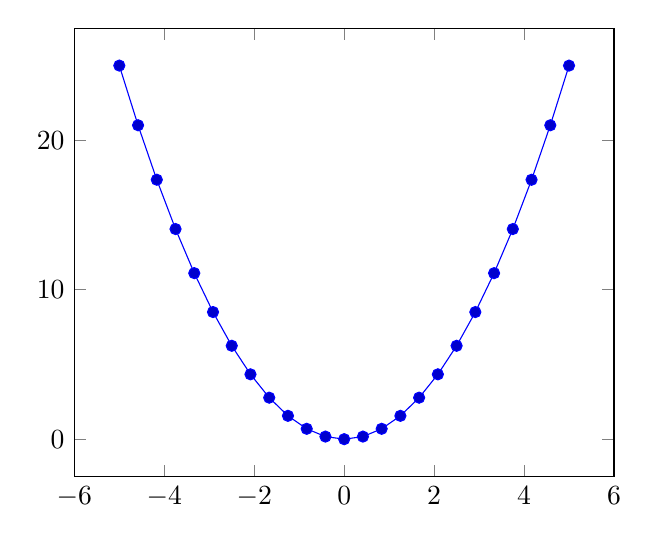
\begin{tikzpicture}
		\begin{axis}
			\addplot {x^2};
		\end{axis}
		\end{tikzpicture}
	\caption{Our first external graphics example}
	\end{figure}

	\begin{figure}
		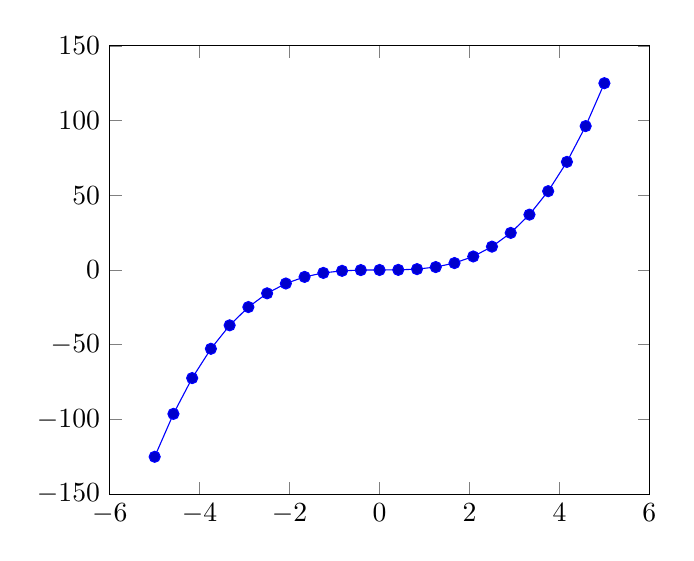
\begin{tikzpicture}
		\begin{axis}
			\addplot {x^3};
		\end{axis}
		\end{tikzpicture}
	\caption{A second graphics}
	\end{figure}
\end{document}
\end{codeexample}
\noindent To enable the system calls, we type
\begin{codeexample}[code only]
pdflatex -shell-escape test
\end{codeexample}
\noindent and \LaTeX\ will now generate the required graphics files |test-figure0.pdf| and |test-figure1.pdf| automatically.

The command |\tikzset{external/force remake}| somewhere in the document can be used to remake every following picture automatically. Of course, it is also possible to simply delete every graphics file.

The library can also be configured to produce a list of figures in case system calls are undesired (or unavailable). In that case, |pdflatex --jobname |\marg{output file name} needs to be invoked for every file name listed in \meta{real file name}|.figlist|. This step can be done within a script.

The command \declareandlabel{\tikzsetexternalprefix}\marg{file prefix} can be used to prepend a directory name to every figure, for example with
\begin{codeexample}[code only]
\tikzsetexternalprefix{figures/}
\end{codeexample}
\noindent to produce |figures/test-figure0.pdf| and |figures/test-figure1.pdf| in our example.

The complete reference documentation and remaining options are documented in the documentation for the ``PDF externalization library'' of~\cite{tikz}. This reference also contains information about how to typeset such a document without \pgfname\ installed or how to provide work-arounds with |.pdf| images and bounding box restrictions.
\index{External Graphics!Bounding Box Issues}
\index{Bounding Box Control!Image Externalization Problems}

\subsection{Exporting Mesh Data From Matlab To \PGFPlots}
While it is easy to write Matlab vectors to files (using |save P.dat data -ASCII|), it is more involved to export mesh data.

The main problem is to communicate the mesh structure to \PGFPlots.

Here is an example how to realize this task: in Matlab, we have mesh data |X|, |Y| and |Z| which are matrizes of the same size. For example, suppose we have

\begin{codeexample}[code only]
[X,Y] = meshgrid( linspace(-1,1,5), linspace(4,5,10) );
Z = X + Y;
surf(X,Y,Z)
\end{codeexample}
\noindent as data. Then, we can generate an $N \times 3$ table containing all single elements in column--wise ordering with

\begin{codeexample}[code only]
data = [ X(:) Y(:) Z(:) ]
save P.dat data -ASCII
\end{codeexample}
\noindent where the second command stores the $N \times 3$ table into |P.dat|. Finally, we can use 

|\addplot3[surf,mesh/rows=10,mesh/ordering=colwise,shader=interp] file {P.dat};|

in \PGFPlots\ to read this data. We need to provide either the number of rows ($10$ here) or the number of columns -- and the ordering (which is |colwise| for Matlab matrizes).

An alternative which is faster in \PGFPlots\ would be to transpose the matrizes in Matlab and tell \PGFPlots\ they are in |rowwise| ordering. So, the last step becomes

\begin{codeexample}[code only]
XX=X'; YY=Y'; ZZ=Z';
data = [ XX(:) YY(:) ZZ(:) ]
save P.dat data -ASCII
\end{codeexample}
\noindent with \PGFPlots\ command

|\addplot3[surf,mesh/cols=10,mesh/ordering=rowwise,shader=interp] file {P.dat};|.

\subsection{matlab2pgfplots.m}
This is a Matlab (tm) script which attempts to convert a matlab figure to \PGFPlots. It requires Matlab version 7.4 (or higher).

The idea is to
\begin{itemize}
	\item use a complete matlab figure as input,
	\item acquire axis labels, axis scaling (log or normal) and legend entries,
	\item acquire all plot coordinates
\end{itemize}
and write an equivalent \texttt{.pgf} file which typesets the plot with \PGFPlots.

The indention is \emph{not} to simulate matlab. It is a first step for a conversion. Type
\begin{lstlisting}
> help matlab2pgfplots
\end{lstlisting}
on your matlab prompt for more information about its features and its limitations.

This script is experimental.

\subsection{matlab2pgfplots.sh}
A \texttt{bash}-script which simply starts matlab and runs 
\begin{lstlisting}
	f=hgload( 'somefigure.fig' );
	matlab2pgfplots( 'outputfile.pgf', 'fig', f );
\end{lstlisting}
See matlab2pgfplots.m above.

\subsection{SVG Output}
It is possible to write every single \Tikz\ picture into a scalable vector graphics (\texttt{.svg}) file. This has nothing to do with \PGFPlots, it is a separate driver of \PGF. Please refer to~\cite[Section ``Producing HTML / SVG Output'']{tikz}.
